%TC:ignore
\section{System's Perspective}
% A description and illustration of the:
\subsection{Design and Architecture of our ITU-MiniTwit System}
%TC:endignore

Our Minitwit application consists of two parts, a User Interface and an API, running in a Docker Swarm \cite{docker_swarm_docs} on DigitalOcean \cite{digitalocean_docs} provisioned by Terraform \cite{terraform_docs}. Data is stored in a PostgreSQL \cite{postgresql_official} database. 
\\
We had a brainstorming session where we discussed what languages could be considered for refactoring. 
Constraints for the chosen language was it should be stable, well established in the industry, with extensive documentation and an active community. \\
The following languages were proposed: Julia, Rust, JavaScript, Nim, Ruby, Elixir and Go.
Using Dot Voting \cite{lucid_dot_voting}, the choice was narrowed down to JavaScript and Ruby which both fulfilled our constraints.
We chose Ruby because we wanted to learn a new language and we liked the simplicity of Ruby-Sinatra \cite{sinatra_docs}. \\
%We chose to deploy on DigitalOcean for monetary reasons, with GitHub Education we could get 200\$ in credits which was more than enough for this project. %Aside from its ease of use, GitHub Actions was also chosen due to its free 2000 minutes / month for a public repository.
The professors initially recommended Vagrant \cite{vagrant_docs} to provision our droplets. When implementing Docker Swarm, we had to replace the Vagrantfile with a bash script (see Section \ref{scaling}), so we knew that we could not revert to Vagrant for our Infrastructure as Code (IaC) solution. We refactored to Terraform because it ensures idempotency by design and is used in the industry.


%TC:ignore
\subsection{Dependencies} % Laurids
%All dependencies of your ITU-MiniTwit systems on all levels of abstraction and development stages. That is, list and briefly describe all technologies and tools you applied and depend on.
% Not needed, not a system dependency %Our system is hosted on Digital Ocean Virtual Machine(s). To keep our service as lightweight and portable as possible we run it entirely within docker containers as illustrated in figure 1.1\textbf{XXX}. % make the stupid graph
%TC:endignore

\begin{figure}[H]
    \centering
    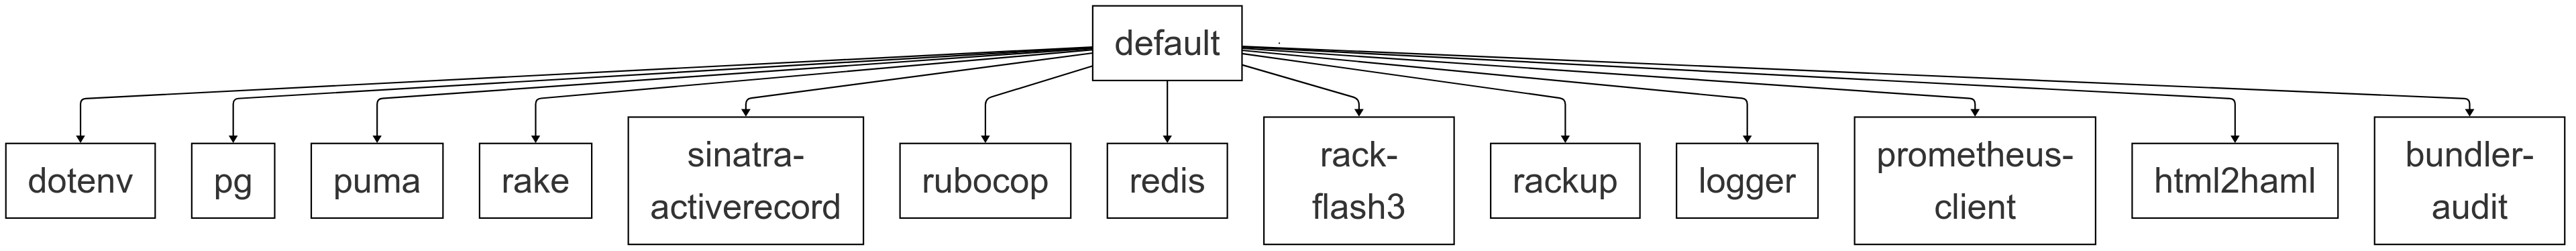
\includegraphics[width=1\linewidth]{images/image.png}
    \caption{Graph of our Gemfile dependencies}
    \label{fig:ruby-deps}
\end{figure}

Our system consists of three parts: a Ruby application, a PostgreSQL database and a Redis database \cite{redis_official}. The Ruby application can be further split into four parts: server, site, data and monitoring, see Figure \ref{fig:ruby-deps} for the dependency tree. For serving our application, we rely on Puma \cite{puma_github} and Rackup \cite{rackup_github}, and, \textit{dotenv} \cite{dotenv} dependencies since we can manage our environment using a \textit{`.env`} file. \\
The application itself is written using Sinatra, chosen for its easy to read documentation and seemingly being the only used alternative to Ruby on Rails. Additionally, we depend on \textit{html2haml} and \textit{haml} for templating our HTML files and \textit{rack-flash3} for pop-ups when accessing our application through the browser. Lastly, we use \textit{bcrypt} \cite{bcrypt_github} to encrypt passwords before storing them. \\
For data management we chose PostgreSQL since it was easier to set up than MySQL. Moving to a Docker Swarm based setup (see Section \ref{section:swarm-setup}), we introduced a Redis cache to keep track of user sessions. Switching database providers was easy using Sequel \cite{sequel}, an object–relational mapping (ORM) library. \\
Finally for monitoring and logging we depend on the \textit{prometheus-client} \cite{prometheus_client_gem} and \textit{logger} \cite{logger160} gems for scraping and logging our application.


% Annoying dependency on the VM when it comes to our database 

\subsection{Interactions of Subsystems}
\begin{figure}[H]
    \centering
    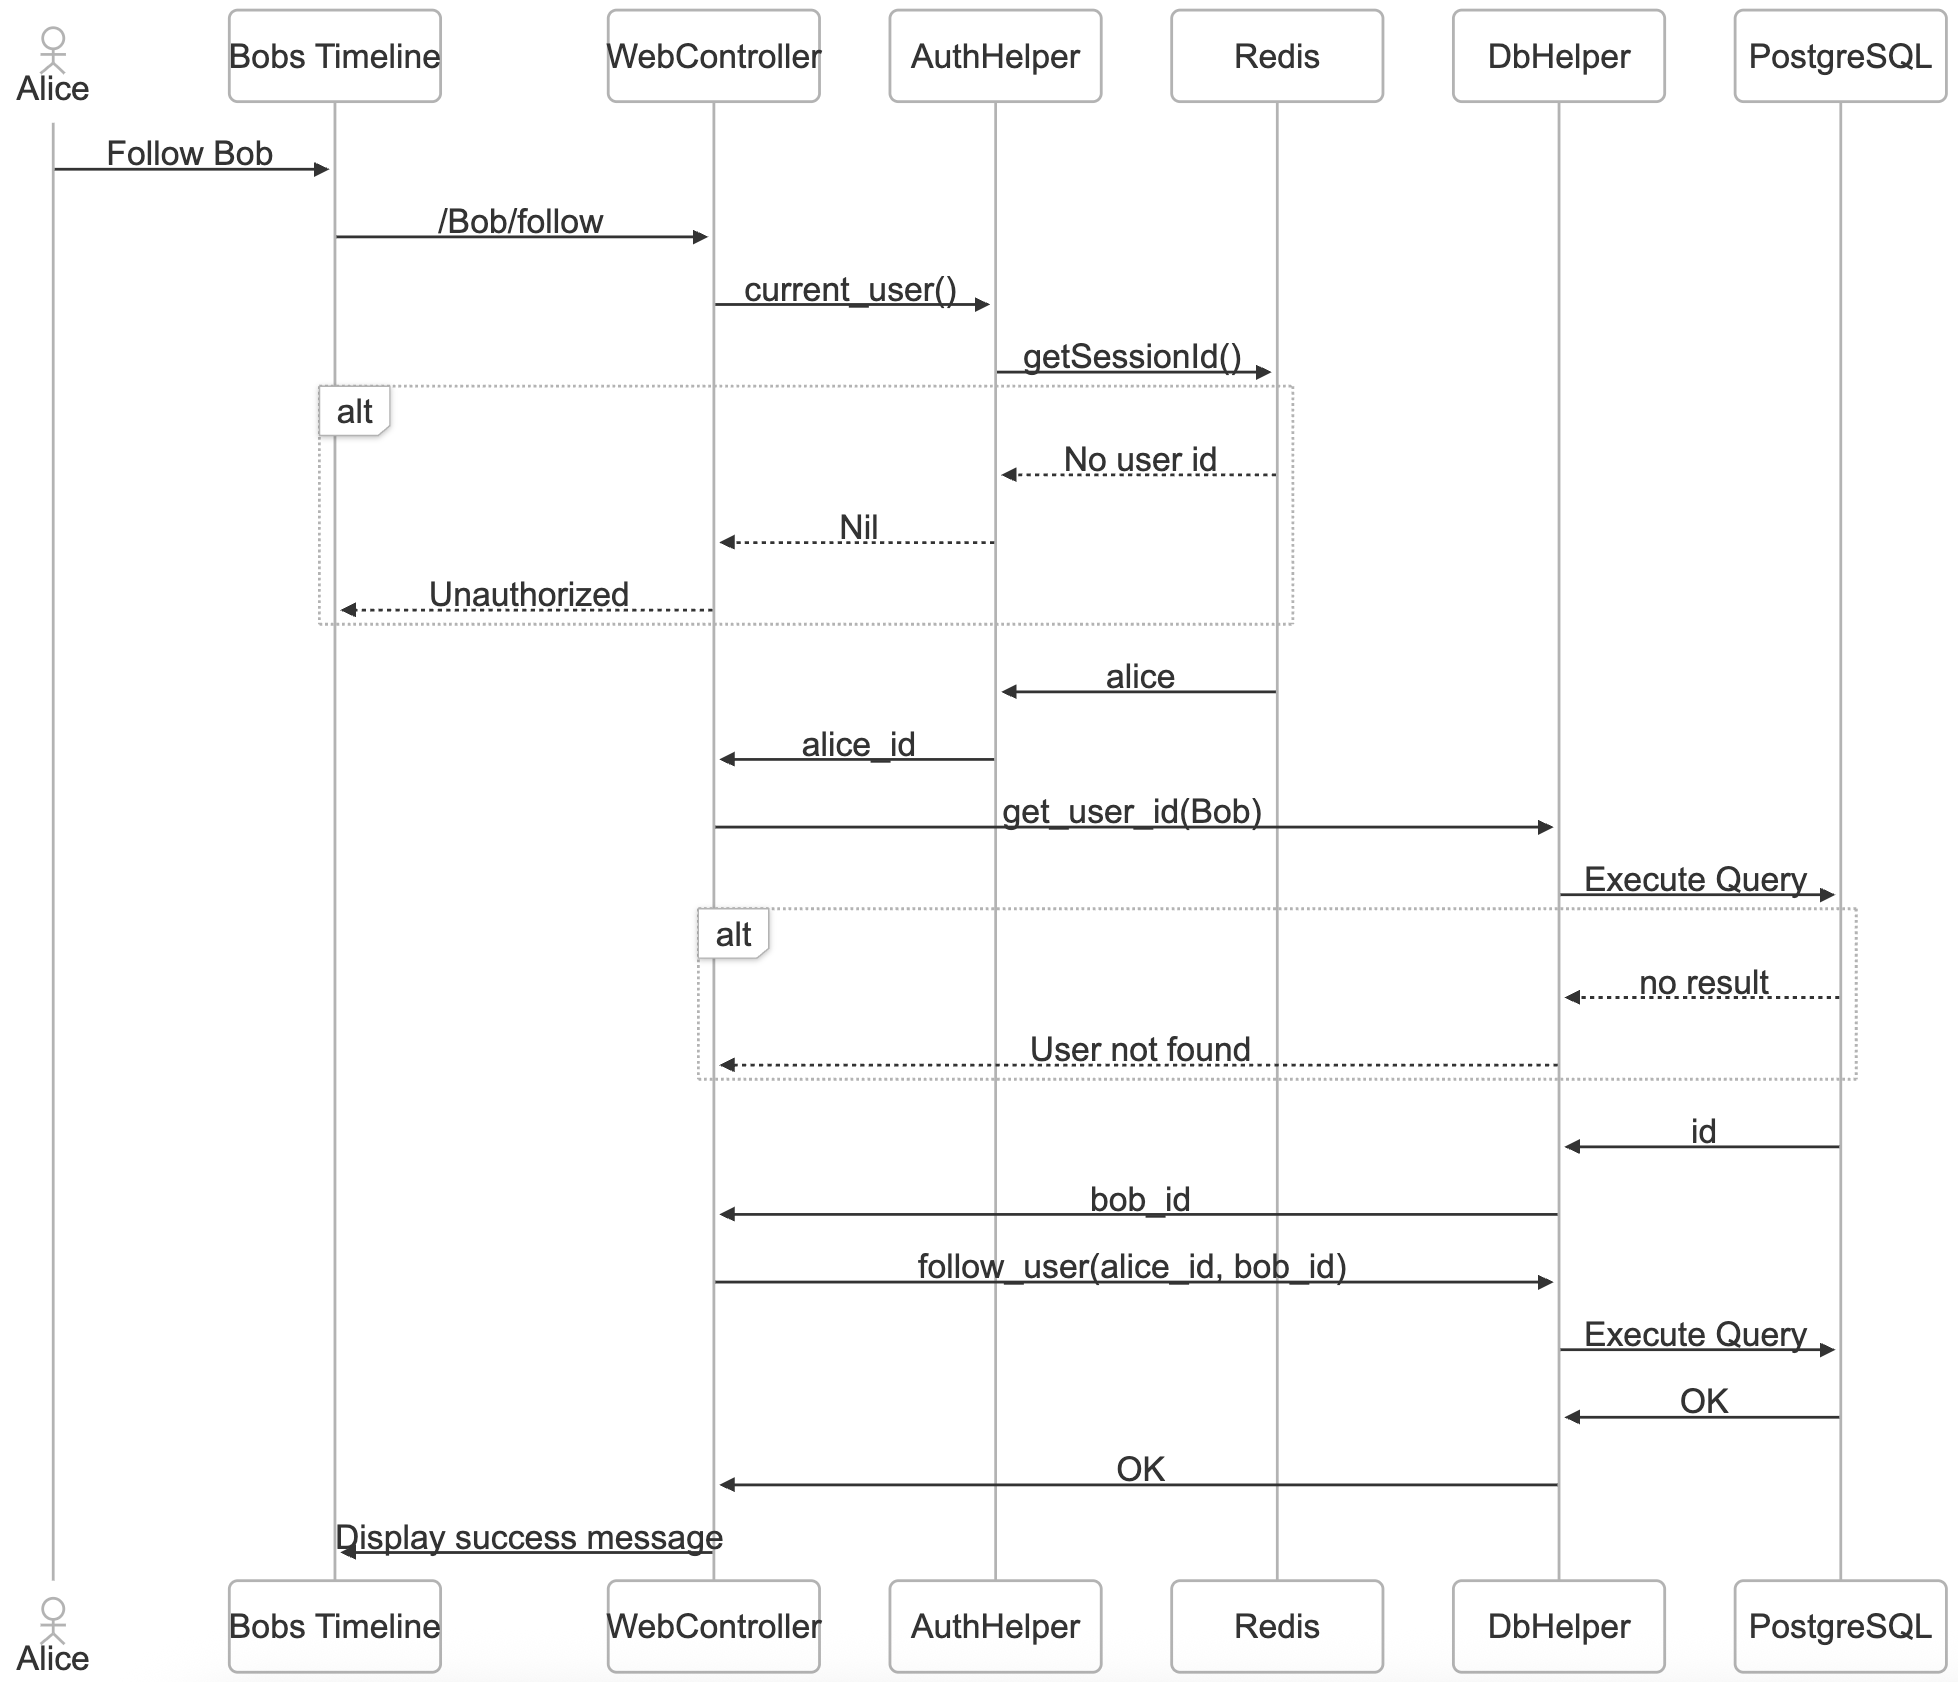
\includegraphics[width=1\linewidth]{images/diagram_user_sequence.png}
    \caption{Sequence diagram of a follow user request traversing our system}
    \label{fig:user_sequence}
\end{figure}

The sequence diagram in Figure \ref{fig:user_sequence} illustrates the process of a user (Alice) initiating a "Follow Bob" action within a web application via the frontend. The WebController is responsible for handling user-initiated actions. For requests, it first ensures that the user is authenticated if required and then delegates to the DbHelper to retrieve or update information. An error message is displayed in the frontend if any errors occur.
\\
\begin{figure}[H]
    \centering
    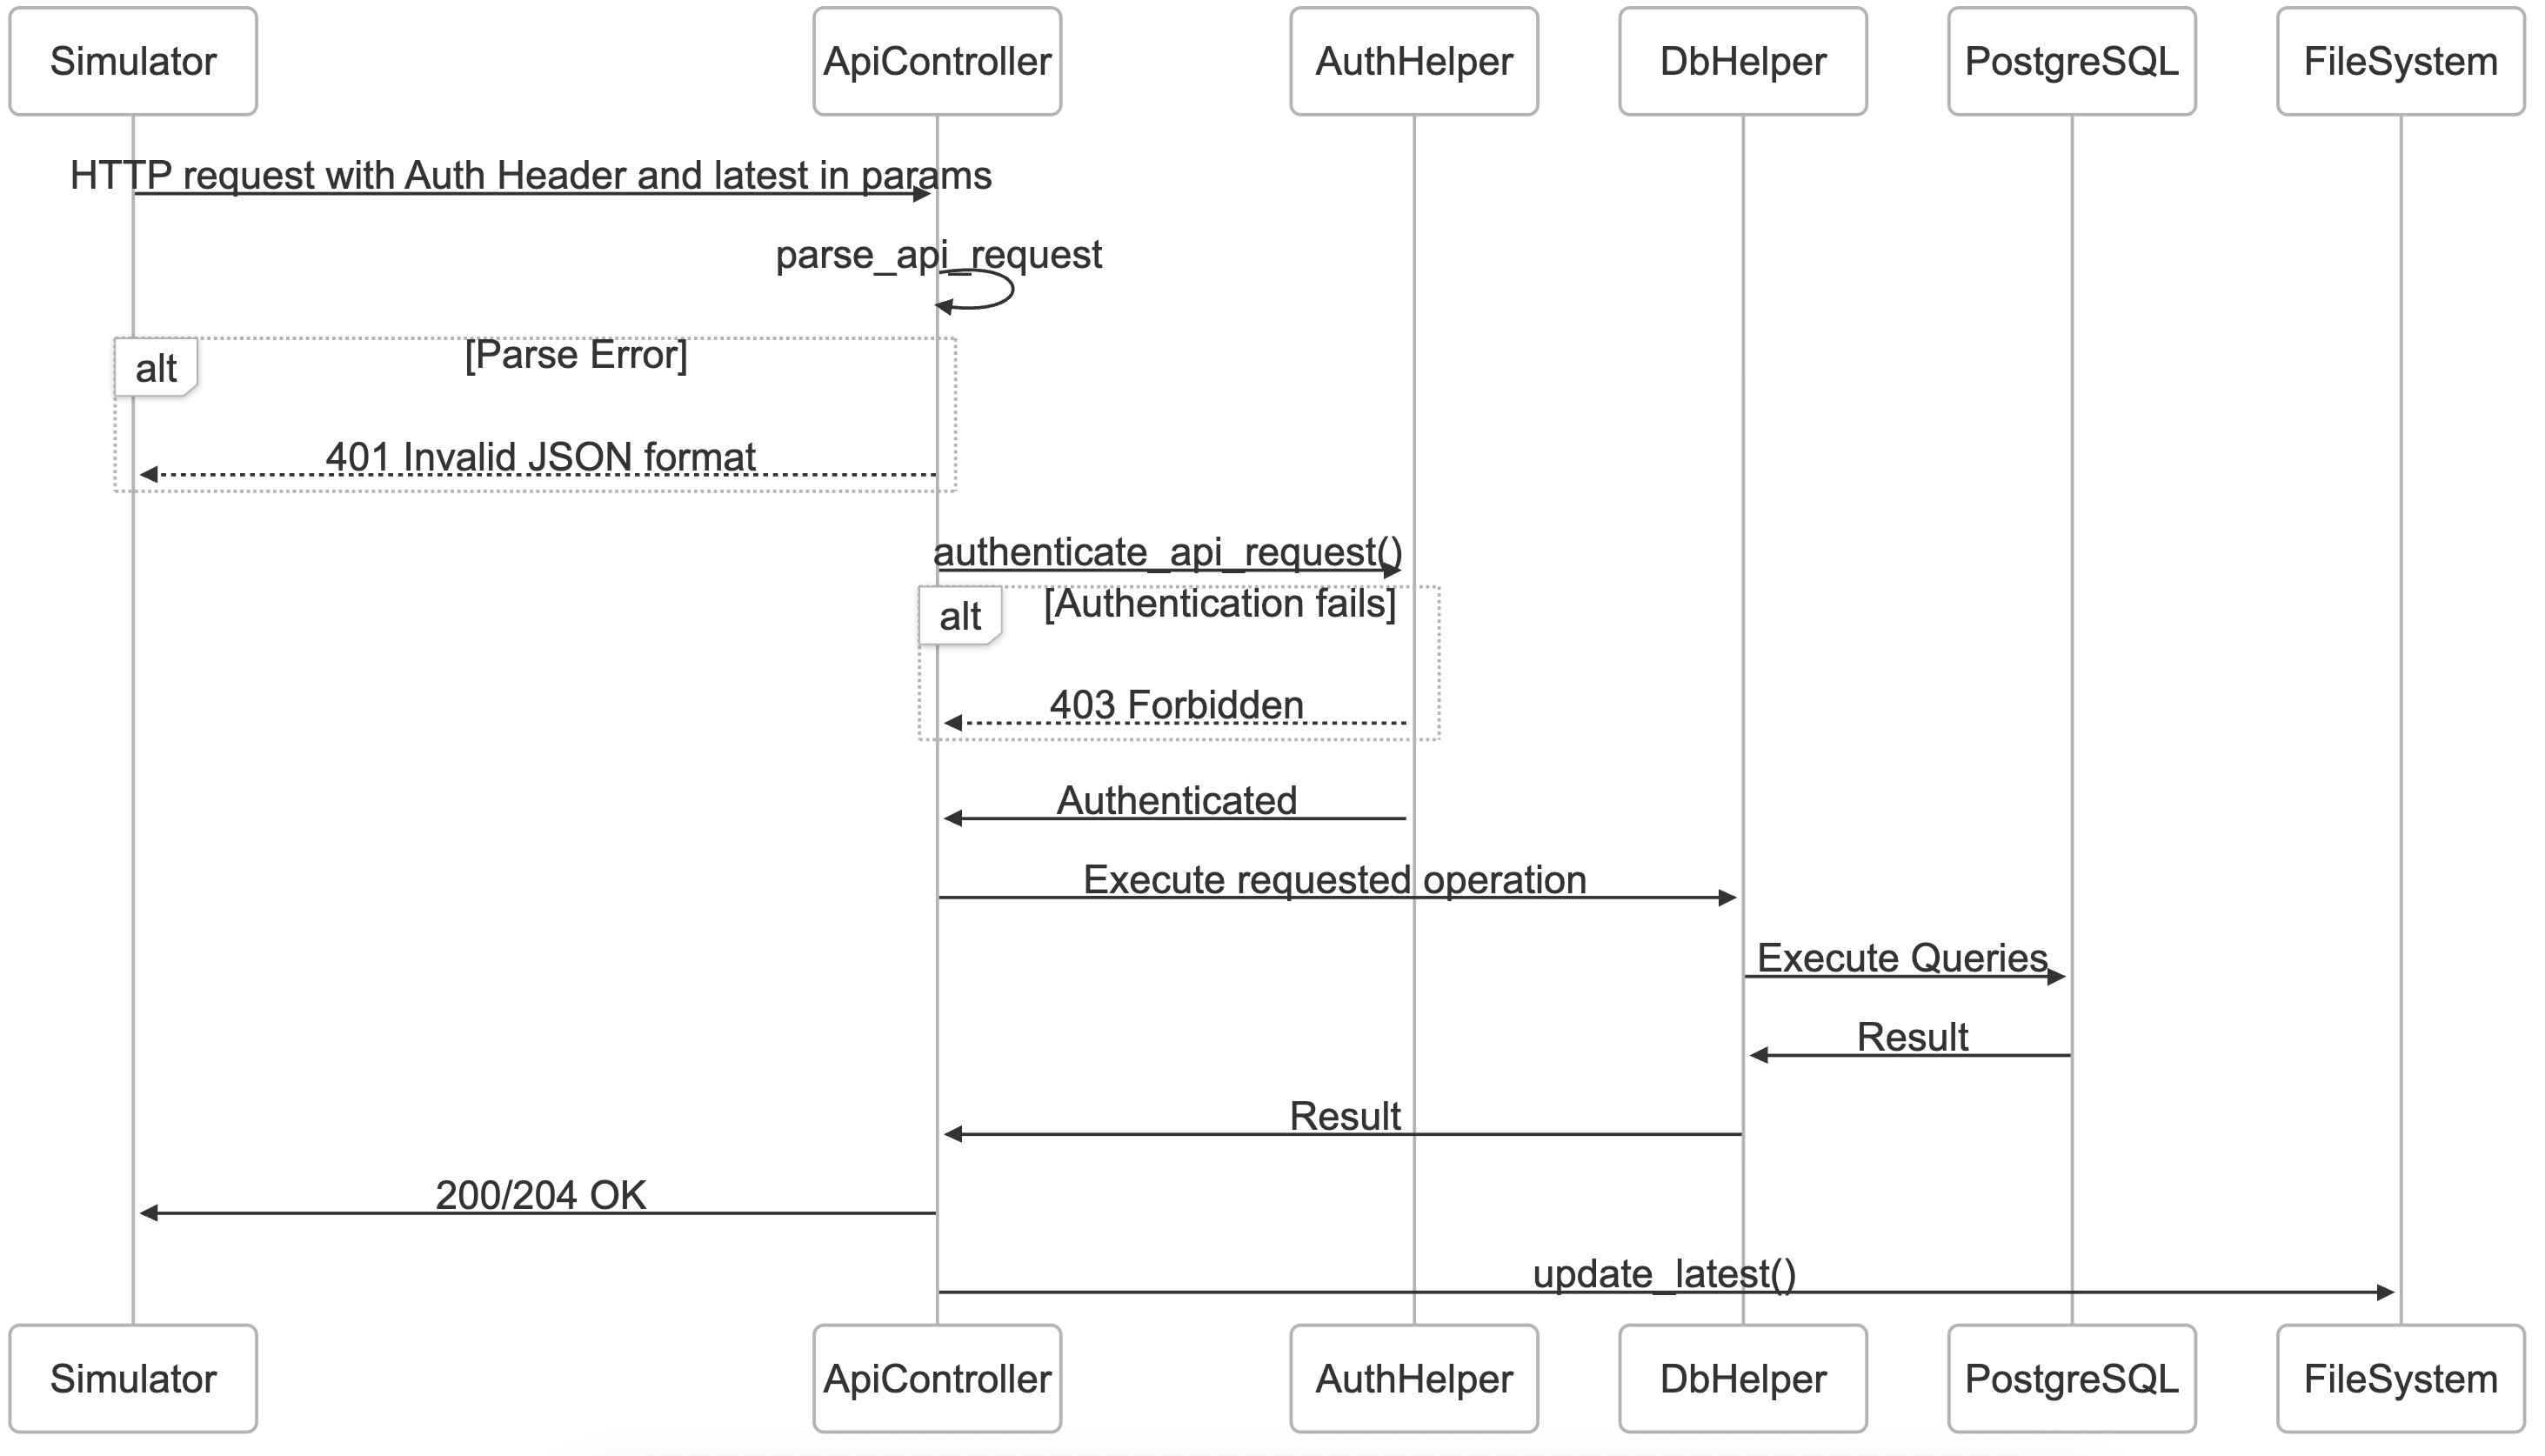
\includegraphics[width=1\linewidth]{images/diagram_sim_sequence.png}
    \caption{Sequence diagram of simulator request traversing our system}
    \label{fig:sim_sequence}
\end{figure}
%
The sequence diagram in Figure \ref{fig:sim_sequence} illustrates an API request originating from the Simulator and received by the APIController. The APIController begins by parsing the parameters and then verifies whether the API key provided in the header is valid. Upon successful authentication, the controller performs the requested operation through the DbHelper, which handles data reads and updates in PostgreSQL. Once the results are retrieved, the controller responds to the Simulator with an appropriate status code and includes the retrieved data in the response body. Finally, the system updates the "latest" state by invoking \texttt{update\_latest()}.
%Important interactions of subsystems.

\subsection{Current State of the System} % Rakul

% static analysis, p. 772, Ian Sommerville:
% Tool-based analysis of a program’s source code to discover errors and anomalies.
% Anomalies, such as successive assignments to a variable with no intermediate use
% may be indicators of programming errors.
% Describe the current state of your systems, for example using results of static analysis and quality assessments.

The following static analysis tools were used throughout the project, in order to improve readability, security and to follow best-practices:
\\
\begin{enumerate}
    \item\textbf{SonarQube} \cite{sonarqube_cloud}: Software as a Service (SaaS) code analysis tool designed to analyse code for maintainability, reliability, and security issues.
    \item\textbf{RuboCop} \cite{rubocop}: A static code analyzer and linter. Enforces many of the guidelines outlined in the community Ruby Style Guide \cite{rubystyleguide}.
    \item \textbf{Bundler Audit} \cite{bundler_audit}: Checks for vulnerabilities in our Ruby dependencies.
    \item\textbf{Hadolint} \cite{hadolint}: Dockerfile linter that helps build best-practice Docker images.
\end{enumerate}
%
SonarQube reports one reliability issue, three security hotspots and one maintainability issue, all deemed low priority by the team (see Appendix \ref{sonarcube-report}).
\\
Some Rubocop rules, such as class length, were disabled due to disrupting developer workflows (see \cite{rubocop_config}). Customizing and enabling the rules would improve the state of the system.
